\documentclass{article}

\usepackage[utf8]{inputenc}
\usepackage{braket}
\usepackage{multirow}
\usepackage{xcolor}
\usepackage[T1]{fontenc}
% \usepackage[french]{babel}
\usepackage{amssymb}
\usepackage{ntheorem}
\usepackage{amsmath}
\usepackage{amssymb}
\usepackage[ a4paper, hmargin={3cm, 3cm}, vmargin={3cm, 3cm}]{geometry}
\usepackage{hyperref}
\usepackage{capt-of}

\usepackage{tikz}
\usetikzlibrary{angles,quotes}

\newcommand{\norm}[1]{\left\lVert#1\right\rVert}

\usepackage{hyperref}
\hypersetup{
    colorlinks,
    citecolor=black,
    filecolor=black,
    linkcolor=blue,
    urlcolor=blue
}

\title{Intro to Quantum Programming \& Alogirthms}
\author{Valeran MAYTIE}
\date{}

\begin{document}
  \maketitle{}

  mail : \href{mailto:benoit.valiron@universte-paris-scalay.fr}
              {       benoit.valiron@universte-paris-scalay.fr}

  \tableofcontents{}

  \section{Introduction}
  \subsection{What is a Quantum systeme}

    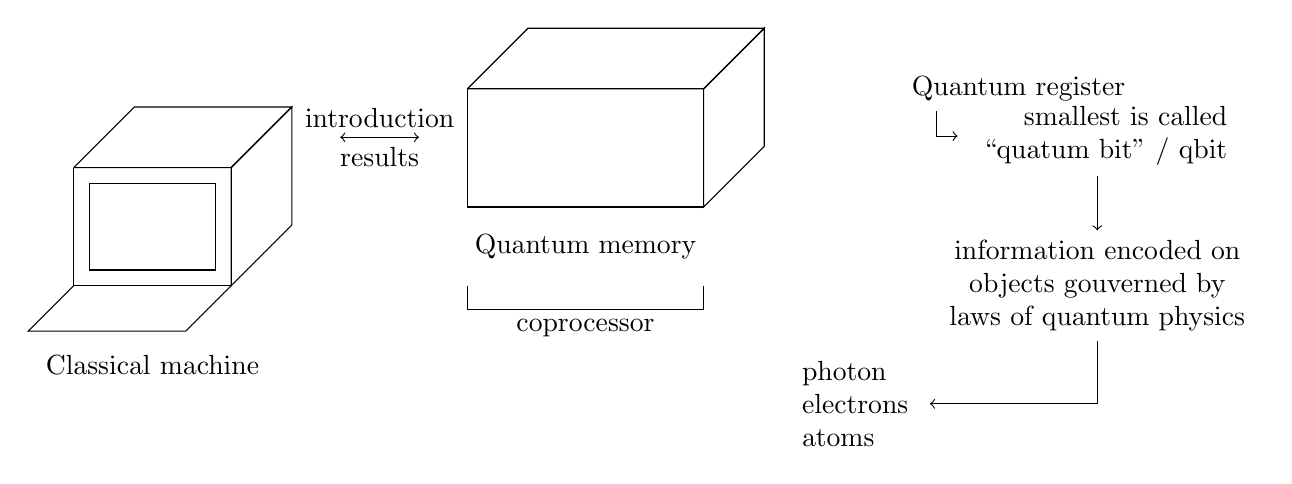
\begin{tikzpicture}
      \draw (0, 0, 0) -- (0, 0, -2) -- (2, 0, -2) -- (2, 0, 0) -- (0, 0, 0);
      \draw (2, 0, 0) -- (2, 0, -2) -- (2, -1.5, -2) -- (2, -1.5, 0) -- (2, 0, 0);
      \draw (0, 0, 0) -- (2, 0, 0) -- (2, -1.5, 0) -- (0, -1.5, 0) -- (0, 0, 0);
      \draw (0.2, -0.2, 0) -- (1.8, -0.2, 0) -- (1.8, -1.3, 0) -- (0.2, -1.3, 0) -- (0.2, -0.2, 0);
      \draw (0, -1.5) -- (0, -1.5, 1.5) -- (2, -1.5, 1.5) -- (2, -1.5);

      \draw (5, 1, 0) -- (5, 1, -2) -- (8, 1, -2) -- (8, 1, 0) -- (5, 1, 0);
      \draw (8, 1, 0) -- (8, 1, -2) -- (8, -0.5, -2) -- (8, -0.5, 0) -- (8, 1, 0);
      \draw (5, 1, 0) -- (8, 1, 0) -- (8, -0.5, 0) -- (5, -0.5, 0) -- (5, 1, 0);

      \draw (5, -1.5) -- (5, -1.8) -- node[below] {coprocessor} (8, -1.8) -- (8, -1.5);

      \draw [<->] (3, 0, -1) -- node [above] {introduction} node [below] {results} (4, 0, -1);

      \node () at (1, -2.5, 0) {Classical machine};
      \node () at (6.5, -1, 0) {Quantum memory};

      \node (Regs) at (12, 1) {Quantum register};
      \node[text width=3.3cm, align=right] (Bit) at (13, 0.4) {smallest is called ``quatum bit'' / qbit};
      \node[text width=4cm, align=center] (Q) at (13, -1.5) {information encoded on objects
        gouverned by laws of quantum physics};

      \node[text width=1.5cm] (L) at (10, -3) {photon electrons atoms};


      \draw[<-] (Bit.west) -| (Regs.195);
      \draw[->] (Bit) -- (Q);
      \draw[->] (Q.south) |- (L.east);
    \end{tikzpicture}
    \captionof{figure}{Quantum system diagram}

    Classically, to encode a \underline{bit} of information you need : \\

    \begin{tabular}{l|c|c}
      item an object & coin & magnet \\
      \hline
      two stats : & \multirow{3}{*}{head / tails} & \multirow{3}{*}{north/south}\\
      - dinstinguishable, & & \\
      - that can be set & & \\
    \end{tabular} \vspace{5mm}

    Quantum : the same ! \\
    \begin{tabular}{c|c|c}
      Object & Photon & electron \\
      \hline
      pair of stats & polarisation V / H & spin up / down \\
      \hline
      \multirow{2}{*}{other pair of states} & one photon &  \\
      & no photon & \\
      \hline
      \multirow{2}{*}{another} & in Fiber A  & \\
      & in Fiber B &
    \end{tabular}

  \subsection{Complex numbers}


    \begin{center}
    \begin{tikzpicture}
      \coordinate (o) at (0, 0);
      \coordinate (a) at (0, 1);
      \coordinate (b) at (1, 0);
      \coordinate (c) at (1, 1);
      \draw[->] (0, -0.5) -- (0, 3);
      \draw[->] (-0.5, 0) -- (3, 0);
      \draw (0, 0) -- node [above, blue] {$\rho$} (2.5, 2.5);
      \node[fill=black,circle,inner sep=1pt]  at (2.5, 2.5) {};

      \node [left, green] at (0, 2.5) {$b$};
      \node [below, orange] at (2.5, 0) {$a$};

      \node [anchor=west] at (5, 3)   {$\theta$ : phases};
      \node [anchor=west] at (5, 2.5) {$\rho$ : magnetude};

      \draw [dotted] (0, 2.5) -- (2.5, 2.5);
      \draw [dotted] (2.5, 0) -- (2.5, 2.5);

      \draw pic[draw, red, "$\theta$" shift={(4mm, 2mm)}, ->] {angle=b--o--c} ;
      
     \end{tikzpicture}
     \captionof{figure}{Complex number representation in diagram}
    \end{center}

    \begin{align*}
      \alpha &= \underbrace{{\color{green}a}+ {\color{orange}b}}_{reals}i &
            \text{is imaginary number } i^2 = -1 \\
      &= {\color{blue}\rho} (\cos {\color{red}\theta} + i \sin {\color{red}\theta}) & \\
      &= {\color{blue}\rho} e^{i\color{red}\theta} \\
    \end{align*}

    Absolute value : $|x| = \rho = \sqrt{a^2 + b^2}$

    Some properties :

    \begin{itemize}
      \item $\overline{a + bi} = a - bi$
      \item $\overline{e^x} = e^{\overline{x}}$
      \item $|\alpha^2| = \rho \times \rho = \alpha \times \overline{\alpha}$
    \end{itemize}

    \begin{center}
    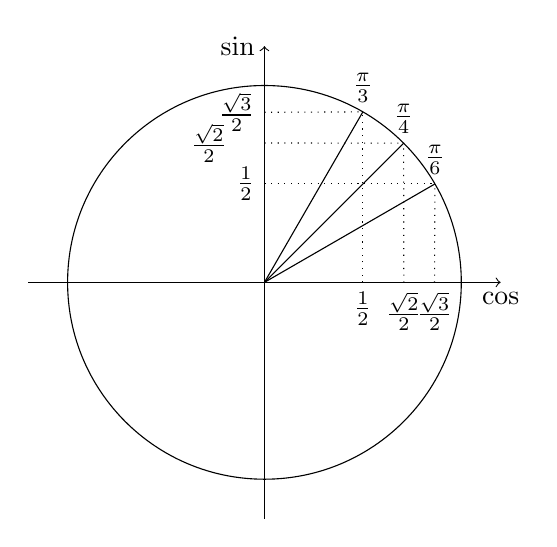
\begin{tikzpicture}
      \draw (0,0) circle (2.5);

      \draw[->] (-3, 0) -- node[pos=1, below] {$\cos$} (3, 0);
      \draw[->] (0, -3) -- node[pos=1, left]  {$\sin$} (0, 3);

      \draw[] (0, 0) -- node[pos=1, above] {$\frac{\pi}{3}$} (60:2.5);
      \draw[] (0, 0) -- node[pos=1, above] {$\frac{\pi}{4}$} (45:2.5);
      \draw[] (0, 0) -- node[pos=1, above] {$\frac{\pi}{6}$} (30:2.5);

      \draw [dotted] (0, 2.16) -- node[pos=0, left]  {$\frac{\sqrt{3}}{2}$} (60:2.5);
      \draw [dotted] (1.25, 0) -- node[pos=0, below] {$\frac{1}{2}$} (60:2.5);

      \draw [dotted] (0, 1.77) -- node[pos=-0.2, left]  {$\frac{\sqrt{2}}{2}$} (45:2.5);
      \draw [dotted] (1.77, 0) -- node[pos=0, below] {$\frac{\sqrt{2}}{2}$} (45:2.5);

      \draw [dotted] (0, 1.25) -- node[pos=0, left]  {$\frac{1}{2}$} (30:2.5);
      \draw [dotted] (2.16, 0) -- node[pos=0, below] {$\frac{\sqrt{3}}{2}$} (30:2.5);

    \end{tikzpicture}
    \end{center}


  \subsection{Hilber Spaces}

    A state of a quantum system is a vector in a Hilbert Space(Finite
    dimenssional) \\
    Two states are distinguishable, it means that they are orhtogonal

    \underline{vector space} :

      \begin{itemize}
        \item pick a set (Finite) call it a ``a basis''
          $\mathcal{B} = \{e_i\}_{i \in I}$

        \item a vector is a linerar combination
          $\alpha_0 e_0 + \alpha_1 e_1 + \ldots + \alpha_{n-1} e_{n-1}$ $\alpha_i \in
          \mathcal{I}$


        \item Scalar product : input 2 vector

          $\langle v|w \rangle = \sum_i \alpha_i \alpha'_i$
      \end{itemize} 

  Hilbert space is a complex vector space with a scalar product

  Let $\mathcal{H}$ be defined by $\{\ket{0}, \ket{1} \}$

  A vector in general : $\alpha \ket{0} + \beta \ket{1}$

  example of orthogonal vectors :

  \begin{align*}
    \ket{0} &\perp \ket{1} \\
    \ket{0} + \ket{1} &\perp \ket{0} - \ket{1}
  \end{align*}

  in a Hilbert space, there is a norm :

  $\norm{v} = \sqrt{\langle u , v \rangle}$

  \subsection{Kronecker product}

  4)

    $\mathcal{E}$ and $\mathcal{F}$ two Hilbert spaces

    build $\mathcal{E} \otimes \mathcal{F}$


    Consider $\mathcal{H} \otimes \mathcal{H}$ a generic elemevector is :

    $\alpha \ket{00} + \beta \ket{01} + \gamma \ket{10} + \delta \ket{11}$

    $\ket{00} \perp$ any other basics element

    Suspose that $v \perp v'$ what about $v \otimes \ket{0}$ and $v' \otimes
    \ket{0}$ ?

  \subsection{Quantum bit}

    The state of a quantum bit is a vector in $\mathcal{H} = \{\alpha \ket{0} +
    \beta \ket{1}\}$

    \begin{itemize}
      \item of norm 1
      \item modulo a global phase
    \end{itemize}

    We say that $v$ and $w$  are relatex by a global phase if exists $\Theta$
    angle such that $v = e^{i\Theta}w$

    \begin{align*}
      v &= \alpha \ket{0} + \beta \ket{1} \\
      w &= \alpha' \ket{0} + \beta' \ket{1}
    \end{align*}

    We can write $v \simeq w$ the state of a qubit is : 
    \begin{itemize}
      \item an equivlence class order $\simeq$ 
      \item a set of vectors classed under multiplication by a global phase
    \end{itemize}


    Consider $\ket{0}$, $e^{i \pi/2}\ket{0}$, $-\ket{0}$ are all represent the
    same qubit because they only differ by an irrelevant global phase.

    Each of then is a representative element of the same qubit state.


    Consider a qubit in state 
    
    \begin{align*}
      \alpha \ket{0} + \beta \ket{1} &= \rho_a e^{i\theta_a} + \rho_b e^{i\theta_b} \ket{1} \\
      &\simeq e^{-i\theta_a}(\rho_a  e^{i\theta_a}  \ket{0} + e^{i\theta_b} \ket{1}) \\
      &= (\rho_a e^{i\theta_a - i \theta_a} \ket{0} + e^{i\theta_b - i\theta_a} \ket{1}) \\
      &= (\rho_a \ket{0} + e^{i\theta} \ket{1}) & \text{with } \theta = \theta_b - \theta_a \\
      &= 5)
    \end{align*}

    a cononical rep element of a qubit state is of the form :

    \begin{align*}
      cos(O / 2) \ket{0} + e^{i\theta} sin(O / 2) \ket{1}
    \end{align*}

    with $O \in [0, \pi]$ and $\theta \in [0, 2\pi[$

    \begin{center}
    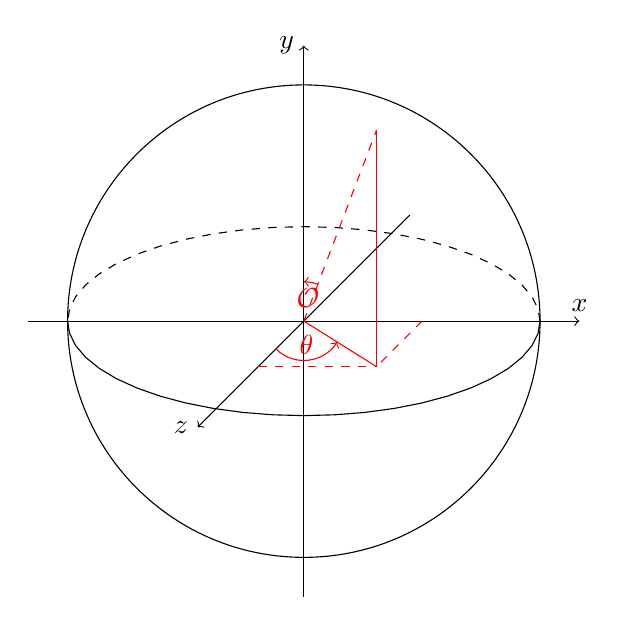
\begin{tikzpicture}
      
      \draw (0, 0) circle(3);
      \draw plot[domain=pi:2*pi] ({3*cos(\x r)},{1.2*sin(\x r)});
      \draw[dashed] plot[domain=0:pi] ({3*cos(\x r)},{1.2*sin(\x r)});

      \draw [->] (-3.5, 0)    -- node[pos=1, above] {$x$} (3.5, 0);
      \draw [->] (0, -3.5)    -- node[pos=1, left ] {$y$} (0, 3.5);
      \draw [->] (0, 0, -3.5) -- node[pos=1, left ] {$z$} (0, 0, 3.5);

      \draw [red, dashed] (1.5, 0)    -- (1.5, 0, 1.5);
      \draw [red, dashed] (0, 0, 1.5) -- (1.5, 0, 1.5);
      \draw [red]         (0, 0)      -- (1.5, 0, 1.5);
    
      \draw [red, dashed] (0, 0)        -- (1.5, 3, 1.5);
      \draw [red]         (1.5, 0, 1.5) -- (1.5, 3, 1.5);

      \coordinate (o) at (0,   0);
      \coordinate (a) at (0,   0, 1.5);
      \coordinate (b) at (1.5, 0, 1.5);
      \draw pic[draw, red, "$\theta$", ->] {angle=a--o--b} ;

      \coordinate (a) at (0,   3, 0);
      \coordinate (b) at (1.5, 3, 1.5);
      \draw pic[draw, red, "$\mathcal{O}$", ->] {angle=b--o--a} ;
    \end{tikzpicture}
    \end{center}

    a quantum bit is instanciated by : 

    \begin{itemize}
      \item a physical object
      \item a pair of othogonal states $\ket{0}$ : false and $\ket{1}$ : true
      \item a state of the qubit is a superposition of $\ket{0}$ and $\ket{1}$
        a linear count of norm 1.
    \end{itemize}

    consider the object $A$ and $B$ coding a qubit and another one $B$ coding a qubitstate in $\mathcal{H}$

    Now join the $2$ systems $A B$ state in $\mathcal{H} \otimes \mathcal{H}$.

    classicaly

    7)

    a 2-qubit system has a state
    $\alpha \ket{00} + \beta \ket{01} + \gamma \ket{10} + \delta \ket{11} $

    one way to build such a system is to :

    \begin{itemize}
      \item generate two separte states

      \item join then $(a \ket 0 + b \ket 1) \otimes (a' \ket 0 + b' \ket 1)=
        aa' \ket{00} + ab' \ket{01} + a'b \ket{10} + a'b' \ket{11}$
    \end{itemize}

    can I reach $\frac{\sqrt{2}}{2}(\ket{00} + \ket{11})$ ? NO ! It is not a
    separable element.

    \vspace{5mm}

    3-qubit state live in $\mathcal{H} \otimes \mathcal{H} \otimes \mathcal{H}$

    8)
    n-qubit
\end{document}
